\documentclass{book}

\usepackage{amsmath}
\usepackage{amssymb}
\usepackage{amsthm}
\usepackage{graphicx}
\usepackage{geometry}
\usepackage{hyperref}
\usepackage{titling}
\usepackage{listings}
\usepackage{array}
\usepackage{mathtools}
\usepackage{bm}
\usepackage{enumerate}

\geometry{a4paper, margin=1in}

\title{Artificial Neural Networks: From Theory to Practice}
\author{A Comprehensive Textbook for Computer Science Students}
\date{\today}

\graphicspath{{../figures/}}

\begin{document}

\maketitle
\tableofcontents

\chapter{Introduction to Machine Learning}
\section{What is Learning?}
Learning is the process of acquiring new knowledge, skills, or behaviors through experience. This process transforms inputs---such as data, experiences, or information---into useful capabilities like expertise, new skills, or predictive models.

\subsection{Core Elements of Learning}
Every learning process involves these fundamental components:
\begin{enumerate}
    \item \textbf{Input}: Data, experiences, or information that enters the learning system
    \item \textbf{Processing}: The manipulation or transformation of that data according to learning rules
    \item \textbf{Output}: The result---new knowledge, skills, or predictive capabilities
    \item \textbf{Feedback}: Information about the effectiveness of learning outcomes
    \item \textbf{Memory}: The ability to retain and access learned information
\end{enumerate}

\subsection{Key Questions in Learning}
\begin{itemize}
    \item What are the essential inputs for the learning process?
    \item How do we measure the effectiveness and success of learning?
    \item What are the underlying mechanisms and processes by which learning occurs?
    \item How can we generalize from specific experiences to handle new situations?
\end{itemize}

\section{What is Reasoning?}
Reasoning is the ability to draw logical conclusions from known facts or learned knowledge. Unlike learning, reasoning relies on logical inference rather than large amounts of data.

\section{Types of Reasoning: Comprehensive Overview}
Understanding different types of reasoning is crucial for designing effective learning systems. Each type has distinct characteristics and applications in both biological and artificial intelligence systems.

\subsection{Inductive Reasoning}
\textbf{Definition:} Inductive reasoning extracts patterns from observed data to make predictions about future or unseen cases. This approach moves from specific observations to general conclusions, yielding probable rather than certain results.

\textbf{Key Characteristics:}
\begin{itemize}
    \item Most prevalent form of reasoning in the animal kingdom and primary mode in machine learning
    \item Forms the basis of most learned behaviors in animals
    \item Used extensively in deep learning and LLMs
    \item Enables generalization from limited examples to broader patterns
\end{itemize}

\subsection{Deductive Reasoning}
\textbf{Definition:} Deductive reasoning moves from general rules and premises to reach specific, guaranteed conclusions. It starts with a general rule and a specific case to reach a logical conclusion.

\textbf{Key Characteristics:}
\begin{itemize}
    \item Provides certainty when premises are true
    \item Animals generally lack this capability for abstract reasoning
    \item LLMs can only mimic this through pattern matching
    \item Forms the basis of formal logic and mathematical proof
\end{itemize}

\subsection{Abductive Reasoning (Inference to Best Explanation)}
\textbf{Definition:} Abductive reasoning starts with an observation and seeks to find the simplest and most likely explanation. It's the process of finding a hypothesis that, if true, would best explain the observation.

\section{Animal Learning}
\subsection{Example: Bait Shyness in Rats}
Rats demonstrate a fundamental learning principle through their feeding behavior:
\begin{itemize}
    \item They sample novel food cautiously
    \item If the food causes illness, they avoid it in the future
    \item Past experience directly informs future decisions
\end{itemize}
This natural learning process parallels challenges in machine learning.

\section{Human Learning: The Cognitive Approach}
Human learning is a complex and multifaceted process that has been studied extensively in psychology and neuroscience. It involves a combination of conscious and unconscious processes, leading to the acquisition of knowledge and skills that are both explicit (declarative) and implicit (procedural).

\subsection{Cognitive Stages of Development}
Jean Piaget's theory of cognitive development provides a classic framework for understanding how learning capabilities evolve from infancy to adulthood.
\begin{itemize}
    \item \textbf{Sensorimotor Stage (0-2 years)}: Learning occurs through sensory experiences and motor interactions with the environment. Object permanence is a key milestone.
    \item \textbf{Preoperational Stage (2-7 years)}: Children begin to think symbolically and use words and pictures to represent objects. Their thinking is egocentric.
    \item \textbf{Concrete Operational Stage (7-11 years)}: Children begin to think logically about concrete events. They grasp concepts like conservation.
    \item \textbf{Formal Operational Stage (12+ years)}: Abstract reasoning and hypothetical thinking emerge.
\end{itemize}
This staged progression suggests that the ability to learn and the types of learning that are possible change fundamentally over a lifetime, a concept that has parallels in the development of more sophisticated machine learning models.

\subsection{The Role of Memory}
Memory is central to learning. The Atkinson-Shiffrin model is a classic theory that proposes three stages of memory:
\begin{enumerate}
    \item \textbf{Sensory Memory:} A very brief buffer for sensory information.
    \item \textbf{Short-Term Memory (Working Memory):} Holds a small amount of information for a short duration. It is where conscious thought and processing occur. This is analogous to the memory (RAM) of a computer.
    \item \textbf{Long-Term Memory:} The vast, semi-permanent storage of knowledge and skills. This is analogous to a computer's hard drive.
\end{enumerate}
The process of moving information from short-term to long-term memory, known as encoding, is critical for learning. Retrieval is the process of accessing this stored information. In machine learning, the "memory" is stored in the model's parameters (weights).

\subsection{Learning Styles and Strategies}
Humans employ a variety of strategies to learn, which can be broadly categorized:
\begin{itemize}
    \item \textbf{Rote learning:} Memorization through repetition (e.g., flashcards). This is similar to overfitting in machine learning, where a model memorizes the training data.
    \item \textbf{Observational learning:} Learning by watching others.
    \item \textbf{Associative learning:} Connecting stimuli or events that occur together in the environment (classical and operant conditioning).
    \item \textbf{Cognitive learning:} Learning through understanding, reasoning, and problem-solving. This is the goal of more advanced AI systems.
\end{itemize}

\section{What is Machine Learning?}
Machine learning is a subfield of artificial intelligence (AI) that provides systems the ability to automatically learn and improve from experience without being explicitly programmed. At its core, machine learning involves developing models that can identify patterns in data and make predictions or decisions based on those patterns.

\subsection{Parallel: Spam Email Filtering}
Consider how biological learning principles apply to spam detection:
\begin{itemize}
    \item \textbf{Naive approach}: Memorize all past spam emails
    \item \textbf{Problem}: Cannot classify previously unseen emails
    \item \textbf{Solution}: Extract generalizable patterns (like words, phrases, or sender patterns)
    \item \textbf{Key insight}: Both rats and spam filters must generalize from specific experiences to handle new, similar situations
\end{itemize}

\section{Types of Machine Learning}
There are three main categories of machine learning algorithms:

\subsection{Supervised Learning}
In supervised learning, the algorithm is trained on a labeled dataset, meaning that each data point is tagged with a correct output. The goal is to learn a mapping function that can predict the output for new, unseen data. Common supervised learning tasks include classification and regression.

\subsection{Unsupervised Learning}
Unsupervised learning deals with unlabeled data. The algorithm tries to learn the underlying structure of the data without any explicit guidance. Common tasks include clustering, dimensionality reduction, and density estimation.

\subsection{Reinforcement Learning}
Reinforcement learning is concerned with how an agent ought to take actions in an environment so as to maximize some notion of cumulative reward. The algorithm learns by trial and error, receiving feedback in the form of rewards or punishments.

\section{The Data and Observation Model}
In machine learning, we typically represent our data as a matrix. Let's denote the dataset as $\mathcal{D}$. A common convention is to represent the data as a design matrix, $X$.

\subsection{The Design Matrix}
The design matrix $X$ is an $m \times n$ matrix, where $m$ is the number of training examples (or observations) and $n$ is the number of features (or variables). Each row of the matrix represents a single data point, and each column represents a feature.

$$ 
 X = \begin{pmatrix}
 x_{11} & x_{12} & \dots & x_{1n} \\
x_{21} & x_{22} & \dots & x_{2n} \\
\vdots & \vdots & \ddots & \vdots \\
x_{m1} & x_{m2} & \dots & x_{mn}
\end{pmatrix}
$$ 

Each row $i$ corresponds to a data point $\mathbf{x}_i^T$, which is a row vector of size $n$.

\section{Probabilistic Model of Learning}
A powerful way to think about machine learning is from a probabilistic perspective. We can think of the learning process as finding a model that best explains the data. This is often framed as finding the parameters $\theta$ of a model that maximize the likelihood of observing the data.

The likelihood function is given by:
$$ 
\mathcal{L}(\theta | X) = P(X | \theta) 
$$ 

The goal of learning is to find the parameters $\hat{\theta}$ that maximize this likelihood. This is known as Maximum Likelihood Estimation (MLE).
$$ 
\hat{\theta}_{MLE} = \arg\max_{\theta} P(X | \theta)
$$ 

\section{Inductive Bias in Machine Learning}
\subsection{What is Inductive Bias?}
\textbf{Definition:} Inductive bias refers to the set of assumptions that a learning algorithm makes to generalize from limited training data to unseen data.

\textbf{Why is it Critical?}
Inductive bias is essential because:
\begin{itemize}
    \item Machine learning models have limited training data
    \item Models must generalize from past observations to unseen cases
    \item Without appropriate bias, models may overfit (memorizing training data without learning generalizable patterns)
    \item All successful learning algorithms require appropriate assumptions about their domain
\end{itemize}

\subsection{Types of Inductive Biases}

\subsubsection{Preference for Simpler Models (Occam's Razor)}
\begin{itemize}
    \item \textbf{Assumption}: Simpler explanations are preferred over complex ones
    \item \textbf{Example}: Decision trees with fewer splits are preferred because they generalize better
    \item \textbf{In Deep Learning}: Regularization techniques (L1, L2) penalize complex models
\end{itemize}

\subsubsection{Smoothness Assumption}
\begin{itemize}
    \item \textbf{Assumption}: Data points that are close together should have similar outputs
    \item \textbf{Example}: In image classification, two similar images should belong to the same class
    \item \textbf{In ML}: K-Nearest Neighbors (KNN) assumes nearby data points have the same label
\end{itemize}

\subsection{Inductive Bias in Specific Architectures}
\subsubsection{Convolutional Neural Networks (CNNs)}
CNNs are designed for image processing and rely on key inductive biases:

\textbf{1. Locality Bias (Local Connectivity)}
\begin{itemize}
    \item \textbf{Assumption}: Nearby pixels are more relevant than distant pixels
    \item \textbf{Example}: In facial recognition, CNN detects eyes, nose, mouth before recognizing entire face
\end{itemize}

\textbf{2. Translation Invariance}
\begin{itemize}
    \item \textbf{Assumption}: An object should be recognized regardless of position
    \item \textbf{How it works}: CNNs use shared convolutional filters
    \item \textbf{Example}: Handwritten digit "3" recognized anywhere in the image
\end{itemize}

\subsubsection{Recurrent Neural Networks (RNNs \& LSTMs)}
RNNs are designed for sequential data and rely on:

\textbf{1. Temporal Dependency Bias}
\begin{itemize}
    \item \textbf{Assumption}: Recent information is more important than distant past
    \item \textbf{Example}: In "The cat sat on the mat", nearby words are more related
\end{itemize}

\subsubsection{Transformers (BERT, GPT)}

\textbf{1. Attention-Based Bias (Self-Attention)}
\begin{itemize}
    \item \textbf{Assumption}: Important words can be anywhere in a sentence
    \item \textbf{Example}: In "The dog chased the ball...which was blue", "which" refers to "ball"
\end{itemize}

\section{Mathematical Foundations of Learning}
\subsection{Learning as Optimization}
Machine learning can be viewed as an optimization problem where we seek to find the best parameters \(\theta\) that minimize a loss function \(L(\theta)\):
\[\theta^* = \arg\min_\theta L(\theta)\]

\subsubsection{Components of a Learning System}
\begin{enumerate}
    \item \textbf{Hypothesis Space} \(\mathcal{H}\): The set of all possible functions the model can represent
    \item \textbf{Loss Function} \(L(\theta)\): Measures how well the model performs on the training data
    \item \textbf{Optimization Algorithm}: Method to find \(\theta^*\) (e.g., gradient descent)
    \item \textbf{Regularization}: Techniques to prevent overfitting and improve generalization
\end{enumerate}

\subsubsection{The Bias-Variance Tradeoff}
The expected prediction error can be decomposed as:
\[\text{Error} = \text{Bias}^2 + \text{Variance} + \text{Irreducible Error}\]
where:
\begin{itemize}
    \item \textbf{Bias}: Error due to simplifying assumptions in the model
    \item \textbf{Variance}: Error due to sensitivity to small fluctuations in training data
    \item \textbf{Irreducible Error}: Inherent noise in the data
\end{itemize}

\subsection{PAC Learning Framework}
\textbf{Probably Approximately Correct (PAC)} learning provides theoretical foundations for when learning is possible.

A concept class \(\mathcal{C}\) is PAC-learnable if there exists an algorithm that, for any distribution \(\mathcal{D}\) and any \(\epsilon, \delta > 0\), can find a hypothesis \(h\) such that:
\[\Pr[\text{error}(h) \leq \epsilon] \geq 1 - \delta\]
using polynomially many samples and computational steps.

\section{Symbolic AI vs Machine Learning}
\subsection{What is Symbolic AI?}
Also known as \textbf{Good Old-Fashioned AI (GOFAI)}, it represents knowledge using symbols, rules, and logic. It uses explicitly programmed rules for reasoning.

\subsection{Symbolic AI vs Machine Learning Comparison}
\begin{table}[h!]
\centering
\begin{tabular}{|l|l|l|}
\hline
\textbf{Feature} & \textbf{Symbolic AI} & \textbf{Machine Learning} \\
\hline
Knowledge Source & Rules \& logic & Data \& patterns \\
Interpretability & Highly explainable & Often a black box \\
Adaptability & Rigid (manual updates) & Can generalize from data \\
Data Requirements & Minimal & Requires large datasets \\
Best Use Cases & Theorem proving & NLP, computer vision \\
\hline
\end{tabular}
\caption{Comparison of Symbolic AI and Machine Learning.}
\end{table}

\chapter{Foundations of Computation}
\section{What is Computation?}
\textbf{Computation} is the process of performing calculations, manipulating data, or executing a sequence of operations to solve problems or transform inputs into desired outputs. It encompasses both the theoretical and practical aspects of processing information.

\section{Computational Models: Theoretical Foundations}
A \textbf{computational model} is a mathematical or conceptual framework that defines how computation is carried out. For an arbitrary computing model, the following metaphoric expression has been proposed:
\begin{center}
    \textbf{computation = storage + transmission + processing}
\end{center}

\section{Four Fundamental Computational Models}

\subsection{Turing Machine (Alan Turing, 1936)}
\textbf{The Foundation of Algorithmic Computation}

\subsubsection{Core Characteristics}
\begin{itemize}
    \item \textbf{Style}: Imperative / mechanical model of computation
    \item \textbf{Core Idea}: A machine reads/writes symbols on an infinite tape with a finite set of rules
    \item \textbf{Representation}:
    \begin{itemize}
        \item Infinite tape divided into cells
        \item Head that can read/write and move left or right
        \item Finite state machine controlling transitions
    \end{itemize}
\end{itemize}

\subsubsection{Strengths and Limitations}
\textbf{Strengths}:
\begin{itemize}
    \item Canonical model for algorithmic computability
    \item Basis of the Church---Turing Thesis
    \item Directly models sequential execution
\end{itemize}

\textbf{Limitations}:
\begin{itemize}
    \item Low-level, not efficient
    \item Sequential by nature, doesn't capture parallelism well
\end{itemize}

\textbf{Example}: A Turing Machine can simulate any algorithm you'd run on a modern computer (given enough tape).

\subsection{Lambda Calculus (Alonzo Church, 1930s)}
\textbf{The Foundation of Functional Computation}

\subsubsection{Core Characteristics}
\begin{itemize}
    \item \textbf{Style}: Functional model of computation
    \item \textbf{Core Idea}: Everything is a function. Computation = function application + substitution
    \item \textbf{Representation}:
    \begin{itemize}
        \item Variables (\texttt{x})
        \item Function definitions (\texttt{$\lambda$x. expression})
        \item Function application (\texttt{(f x)})
    \end{itemize}
\end{itemize}

\subsubsection{Strengths and Limitations}
\textbf{Strengths}:
\begin{itemize}
    \item Basis of functional programming (Haskell, Lisp)
    \item Good for reasoning about higher-order functions, abstraction, recursion
\end{itemize}

\textbf{Limitations}:
\begin{itemize}
    \item Abstract and symbolic; not naturally tied to hardware
    \item Efficiency is not modeled, just computability
\end{itemize}

\textbf{Example}: Addition can be defined entirely in terms of functions (Church numerals).

\subsection{Cellular Automata (Stanislaw Ulam, John von Neumann, later Conway)}
\textbf{The Foundation of Distributed/Parallel Computation}

\subsubsection{Core Characteristics}
\begin{itemize}
    \item \textbf{Style}: Spatial / distributed model of computation
    \item \textbf{Core Idea}: Computation arises from simple local rules applied to a grid of cells over time
    \item \textbf{Representation}:
    \begin{itemize}
        \item Infinite (or finite) grid of cells
        \item Each cell has a finite state (e.g., alive/dead)
        \item Transition rules depend only on the local neighborhood
    \end{itemize}
\end{itemize}

\subsubsection{Strengths and Limitations}
\textbf{Strengths}:
\begin{itemize}
    \item Good for modeling parallel, distributed, physical systems
    \item Supports universal computation (Conway's Life is Turing-complete)
\end{itemize}

\textbf{Limitations}:
\begin{itemize}
    \item Not natural for symbolic or algebraic computation
    \item More suited for simulating dynamics
\end{itemize}

\textbf{Example}: Conway's \textit{Game of Life} shows how simple rules produce complex, even universal, behaviors.

\subsection{Biological Computation (Inspired by Nature)}
\textbf{The Foundation of Adaptive/Learning Computation}

\subsubsection{Core Characteristics}
Biological models are inspired by living systems and emphasize parallelism, adaptability, and learning.
\begin{itemize}
    \item \textbf{Learns from data} (training) rather than using fixed rules
    \item Massive parallelism and fault tolerance
    \item Self-organization and adaptation
    \item Pattern recognition and generalization
\end{itemize}

\subsubsection{Examples of Biological Computation}
\textbf{Neural Networks}:
\begin{itemize}
    \item Inspired by the brain's neurons and synapses
    \item Computation happens through weighted sums and nonlinear activations
    \item Foundation of modern AI (deep learning for vision, NLP, etc.)
\end{itemize}

\textbf{DNA Computing}:
\begin{itemize}
    \item Uses DNA strands and biochemical reactions to encode and solve problems
    \item Enables massive parallelism (billions of molecules interacting at once)
    \item Example: Adleman (1994) solved a small Hamiltonian Path problem with DNA
\end{itemize}

\textbf{Swarm Intelligence}:
\begin{itemize}
    \item Inspired by ants, bees, and bird flocks
    \item Simple agents interacting lead to complex global solutions
    \item Example: Ant Colony Optimization for shortest path problems
\end{itemize}

\section{Biological Neural Networks: Nature's Computational Model}
The following are key characteristics that make biological neural networks powerful computational systems:

\subsection{Characteristics of Biological Neural Networks}
\begin{itemize}
    \item \textbf{Highly interconnected:} Neurons form a complex web of connections
    \item \textbf{Robustness and Fault Tolerance:} The decay of nerve cells does not affect the overall function of the network significantly
    \item \textbf{Flexibility:} The ability to reorganize and adapt to new situations
    \item \textbf{Handling incomplete information:} Ability to infer appropriate outputs even when some inputs are missing or noisy
    \item \textbf{Parallel processing:} Multiple neurons can process information simultaneously
\end{itemize}
\subsection{Neuron Structure}
\begin{figure}[h!]
\centering
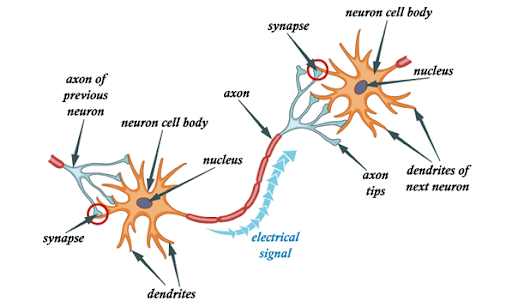
\includegraphics[width=0.8\textwidth]{biological_neuron.png}
\caption{Structure of a biological neuron.}
\end{figure}
\subsection{Neuron Structure and Components}
\begin{itemize}
    \item \textbf{Fundamental unit}: neuron (cell body / soma, dendrites, axon, synapses)
    \item \textbf{Dendrites} receive inputs; \textbf{axon} transmits output and branches to many synapses (often thousands)
    \item \textbf{Synapse}: junction between axon terminal and target cell
    \item \textbf{Synaptic junctions} form between presynaptic axon terminals and postsynaptic dendrites or the cell body
\end{itemize}

\subsubsection{Typical Sizes}
\begin{itemize}
    \item soma $\sim$ 10--80 $\mu$m
    \item synaptic gap $\sim$ 200 nm
    \item neuron length from 0.01 mm to 1 m
\end{itemize}

\subsection{Signal Transmission and Firing}
\begin{itemize}
    \item \textbf{Resting potential} $\sim$ -70 mV; depolarization above threshold (roughly $\sim$10 mV) triggers firing
    \item \textbf{Action potentials} are all-or-none pulses sent down the axon; information is encoded in firing rate ($\sim$1--100 Hz)
    \item \textbf{Propagation speed} in brain tissue $\sim$ 0.5--2 m/s; synaptic transmission delay $\sim$ 0.5 ms
    \item After firing the membrane recovers (\textbf{refractory period}); synaptic effects decay with time constant $\sim$5--10 ms
\end{itemize}

\subsection{Synapses: Chemistry and Types}
\begin{itemize}
    \item \textbf{Transmission} across synapse is chemical: neurotransmitters released from presynaptic terminal
    \item \textbf{Postsynaptic effect} can be excitatory (depolarizing) or inhibitory (hyperpolarizing)
    \item All endings of a given axon are typically either excitatory or inhibitory
    \item \textbf{Synaptic strength} depends on activity and can change over time (basis for learning)
\end{itemize}



\subsection{Plasticity and Learning}
Active synapses that repeatedly contribute to postsynaptic firing tend to strengthen; inactive ones weaken. \textbf{Hebb's rule} ("cells that fire together, wire together") describes this activity-dependent plasticity. Continuous modification of synaptic strengths underlies learning and memory formation.

\section{Artificial Neural Networks}
\subsection{Introduction: From Biology to Computation}
Artificial Neural Networks (ANNs) represent one of the most successful attempts to harness the computational principles observed in biological neural systems for solving complex problems.

\subsection{The Abstract Neuron: Building Block of Intelligence}
The output of a neuron can be expressed as:
\[ Y = f\left(\sum_{i=1}^{n} W_i X_i + b\right) = f(\mathbf{W}^T \mathbf{X} + b)\]
Where:
\begin{itemize}
    \item \(Y\): Output of the neuron
    \item \(f\): Activation function (primitive function that introduces non-linearity)
    \item \(W_i\): Weight associated with input \(i\) (learnable parameter)
    \item \(X_i\): Value of input \(i\)
    \item \(b\): Bias term (learnable parameter that shifts the activation function)
    \item \(\mathbf{W} = [W_1, W_2, \ldots, W_n]^T\): Weight vector
    \item \(\mathbf{X} = [X_1, X_2, \ldots, X_n]^T\): Input vector
\end{itemize}

\subsubsection{Mathematical Foundation: Linear Combination and Affine Transformation}
The computation \(\mathbf{W}^T \mathbf{X} + b\) represents an \textbf{affine transformation} of the input space. This can be broken down as:
\begin{enumerate}
    \item \textbf{Linear transformation}: \(\mathbf{W}^T \mathbf{X}\) scales and rotates the input vector
    \item \textbf{Translation}: Adding bias \(b\) shifts the result by a constant
\end{enumerate}

The activation function \(f\) then introduces non-linearity, enabling the neuron to model complex, non-linear relationships between inputs and outputs.

\section{Activation Functions: Mathematical Properties}
Activation functions are crucial for introducing non-linearity into neural networks. Different activation functions have distinct mathematical properties that affect learning dynamics.

\subsection{Common Activation Functions}
\subsubsection{Step Function (Heaviside)}
\[\phi(z) = \begin{cases} 1 & \text{if } z \geq 0 \\ 0 & \text{if } z < 0 \end{cases}\]
\textbf{Properties}: Non-differentiable, binary output, historically important for perceptron.

\subsubsection{Sigmoid Function}
\[\sigma(z) = \frac{1}{1 + e^{-z}}\]
\textbf{Properties}:
\begin{itemize}
    \item Smooth, differentiable: \(\sigma'(z) = \sigma(z)(1 - \sigma(z))\)
    \item Range: \((0, 1)\)
    \item Problem: Vanishing gradients for large \(|z|\)
\end{itemize}

\subsubsection{Hyperbolic Tangent}
\[\tanh(z) = \frac{e^z - e^{-z}}{e^z + e^{-z}} = 2\sigma(2z) - 1\]
\textbf{Properties}:
\begin{itemize}
    \item Range: \((-1, 1)\)
    \item Zero-centered output
    \item Derivative: \(\tanh'(z) = 1 - \tanh^2(z)\)
\end{itemize}

\subsubsection{Rectified Linear Unit (ReLU)}
\[\text{ReLU}(z) = \max(0, z)\]
\textbf{Properties}:
\begin{itemize}
    \item Computationally efficient
    \item Alleviates vanishing gradient problem
    \item Non-differentiable at \(z = 0\)
    \item Can suffer from "dying ReLU" problem
\end{itemize}

\subsection{Mathematical Requirements for Activation Functions}
For universal approximation, activation functions should be:
\begin{enumerate}
    \item \textbf{Non-linear}: Otherwise, multiple layers collapse to a single linear transformation
    \item \textbf{Differentiable}: Enables gradient-based optimization (almost everywhere is sufficient)
    \item \textbf{Monotonic}: Helps with optimization landscape (not strictly required)
    \item \textbf{Bounded or unbounded}: Different properties affect convergence behavior
\end{enumerate}

\subsection{Neural Networks as Function Approximators}
With sufficient neurons and appropriate activation functions, neural networks can approximate any continuous function to arbitrary precision.

\subsubsection{Universal Approximation Theorem}
\textbf{Theorem (Cybenko, 1989; Hornik, 1991)}: Let \(\phi\) be a continuous sigmoid-type function. Then finite sums of the form:
\[F(x) = \sum_{j=1}^{N} \alpha_j \phi(y_j^T x + \theta_j)\]
are dense in \(C(I_n)\), the space of continuous functions on the unit hypercube \(I_n = [0,1]^n\).

\subsubsection{Implications}
\begin{itemize}
    \item \textbf{Existence}: There exists a neural network that can approximate any continuous function
    \item \textbf{No constructive proof}: Doesn't tell us how to find the network
    \item \textbf{Width vs. Depth}: Original theorem about width; depth can be more efficient
    \item \textbf{Approximation vs. Learning}: Says nothing about learnability from data
\end{itemize}

\subsubsection{Modern Extensions}
\begin{itemize}
    \item \textbf{ReLU networks}: Also have universal approximation properties
    \item \textbf{Deep vs. Wide}: Deep networks can be exponentially more efficient than wide ones
    \item \textbf{Smooth functions}: Require fewer neurons than general continuous functions
\end{itemize}

\section{Artificial Neural Networks: From Theory to Implementation}

\subsection{Fundamental Architecture: Primitive Functions and Composition Rules}
To understand artificial neural networks, we must first examine their core computational elements. Every computational model requires:
\begin{enumerate}
    \item \textbf{Primitive Functions}: Basic operations that cannot be decomposed further
    \item \textbf{Composition Rules}: Ways to combine primitive functions to create complex behaviors
\end{enumerate}

\subsubsection{Primitive Functions in Neural Networks}
In artificial neural networks, \textbf{primitive functions are located in the nodes (neurons) of the network}. Each node implements a specific mathematical transformation that processes incoming information and produces an output.

\subsubsection{Composition Rules in Neural Networks}
The \textbf{composition rules are contained implicitly in}:
\begin{itemize}
    \item \textbf{Interconnection pattern of the nodes}: How neurons are connected determines information flow
    \item \textbf{Synchrony or asynchrony of information transmission}: Whether neurons update simultaneously or in sequence
    \item \textbf{Presence or absence of cycles}: Whether information can flow in loops (recurrent networks) or only forward (feedforward networks)
\end{itemize}

This differs fundamentally from traditional computing models:

\begin{table}[h!]
\centering
\begin{tabular}{|l|l|l|}
\hline
\textbf{Computing Model} & \textbf{Primitive Functions} & \textbf{Composition Rules} \\
\hline
\textbf{von Neumann Processor} & Machine instructions & Program sequence + control flow \\
& (ADD, MOVE, JUMP) & \\
\hline
\textbf{Artificial Neural Networks} & Neuron activation functions & Network topology + connection \\
& & weights + timing \\
\hline
\end{tabular}
\caption{Comparison of primitive functions and composition rules across computing models.}
\end{table}

\subsection{Neural Networks as Function Approximators}

\subsubsection{Networks of Primitive Functions}
\textbf{Artificial neural networks are nothing but networks of primitive functions.} Each node transforms its input into a precisely defined output, and the combination of these transformations creates complex computational behaviors.

\subsubsection{The Network Function}
Consider a neural network that takes inputs $(x, y, z)$ and produces an output through nodes implementing primitive functions $f_1, f_2, f_3, f_4$. The network can be thought of as implementing a \textbf{network function} $\phi$:
\[\phi(x, y, z) = f_4(a_4 \cdot f_3(a_3 \cdot f_2(a_2 \cdot f_1(a_1 \cdot x))) + \ldots)\]
Where $a_1, a_2, \ldots, a_5$ are the weights of the network. \textbf{Different selections of weights produce different network functions.}

\subsubsection{Three Critical Elements}
Different models of artificial neural networks differ mainly in three fundamental aspects:
\begin{enumerate}
    \item \textbf{Structure of the Nodes}
    \begin{itemize}
        \item Choice of activation function (sigmoid, ReLU, tanh, etc.)
        \item Input integration method (weighted sum, product, etc.)
        \item Presence of bias terms
    \end{itemize}
    \item \textbf{Topology of the Network}
    \begin{itemize}
        \item Feedforward vs. recurrent connections
        \item Number of layers and neurons per layer
        \item Connection patterns (fully connected, sparse, convolutional)
    \end{itemize}
    \item \textbf{Learning Algorithm}
    \begin{itemize}
        \item Method for finding optimal weights
        \item Supervised vs. unsupervised vs. reinforcement learning
        \item Optimization techniques (gradient descent, evolutionary algorithms)
    \end{itemize}
\end{enumerate}

\subsection{Function Approximation: The Classical Problem}

\subsubsection{Historical Context}
Function approximation is a classical problem in mathematics: \textbf{How can we reproduce a given function $F : \mathbb{R} \rightarrow \mathbb{R}$ either exactly or approximately using a given set of primitive functions?}

Traditional approaches include:
\begin{itemize}
    \item \textbf{Polynomial approximation}: Using powers of $x$ (Taylor series)
    \item \textbf{Fourier approximation}: Using trigonometric functions (sine and cosine)
    \item \textbf{Spline approximation}: Using piecewise polynomials
\end{itemize}

\subsubsection{Neural Networks as Universal Approximators}
Neural networks provide a revolutionary approach to function approximation:

\textbf{Key Insight}: With sufficient neurons and appropriate activation functions, neural networks can approximate any continuous function to arbitrary precision (Universal Approximation Theorem).

\subsubsection{Advantages of Neural Network Approximation}
\begin{enumerate}
    \item \textbf{Adaptive}: Networks learn the approximation from data rather than requiring explicit mathematical formulation
    \item \textbf{Flexible}: Can handle high-dimensional inputs and complex, non-linear relationships
    \item \textbf{Robust}: Can generalize to unseen data and handle noise
    \item \textbf{Parallel}: Multiple neurons can process different aspects of the input simultaneously
\end{enumerate}

\subsection{Learning from Data: The Key Difference}
The main difference between Taylor or Fourier series and artificial neural networks is, however, that \textbf{the function F to be approximated is given not explicitly but implicitly through a set of input-output examples.} We know F only at some points but we want to generalize as well as possible. This means that we try to adjust the parameters of the network in an optimal manner to reflect the information known and to extrapolate to new input patterns which will be shown to the network afterwards. This is the task of the learning algorithm used to adjust the network's parameters.

\subsubsection{Classical Series vs. Neural Networks: A Fundamental Distinction}

\textbf{Classical Mathematical Series (Taylor/Fourier):}
\begin{itemize}
    \item \textbf{Explicit Function Definition}: The function $F(x)$ is mathematically defined and known
    \item \textbf{Analytical Coefficients}: Series coefficients can be computed directly using calculus
    \begin{itemize}
        \item Taylor: $a_n = F^{(n)}(x_0)/n!$ (nth derivative at expansion point)
        \item Fourier: $a_n, b_n$ computed via integration over the function's period
    \end{itemize}
    \item \textbf{Perfect Representation}: Given enough terms, the series can represent the function exactly
    \item \textbf{No Learning Required}: Coefficients are determined mathematically, not learned
\end{itemize}

\textbf{Artificial Neural Networks:}
\begin{itemize}
    \item \textbf{Implicit Function Definition}: The function F is unknown but represented by data points
    \item \textbf{Learned Parameters}: Network weights and biases are learned from examples
    \item \textbf{Approximation from Samples}: Must generalize from finite training data to unknown inputs
    \item \textbf{Adaptive Learning}: Parameters adjust through iterative optimization algorithms
\end{itemize}

\subsubsection{Mathematical Formulation of the Learning Problem}
Given a training dataset \(\mathcal{D} = \{(\mathbf{x}_i, y_i)\}_{i=1}^{m}\), we seek to find parameters \(\boldsymbol{\theta}\) that minimize the empirical risk:
\[\mathcal{R}_{\text{emp}}(\boldsymbol{\theta}) = \frac{1}{m} \sum_{i=1}^{m} L(f(\mathbf{x}_i; \boldsymbol{\theta}), y_i)\]

where:
\begin{itemize}
    \item \(L(\cdot, \cdot)\): Loss function measuring prediction error
    \item \(f(\mathbf{x}; \boldsymbol{\theta})\): Neural network function with parameters \(\boldsymbol{\theta}\)
    \item Goal: Minimize true risk \(\mathcal{R}(\boldsymbol{\theta}) = \mathbb{E}_{(\mathbf{x},y) \sim P}[L(f(\mathbf{x}; \boldsymbol{\theta}), y)]\)
\end{itemize}

\subsubsection{Generalization Gap}
The fundamental challenge is the generalization gap:
\[\text{Generalization Gap} = \mathcal{R}(\boldsymbol{\theta}) - \mathcal{R}_{\text{emp}}(\boldsymbol{\theta})\]

This gap can be controlled through:
\begin{enumerate}
    \item \textbf{Regularization}: Adding penalty terms to control model complexity
    \item \textbf{Cross-validation}: Using held-out data to estimate generalization performance
    \item \textbf{Early stopping}: Halting training before overfitting occurs
    \item \textbf{Data augmentation}: Artificially increasing training set size
\end{enumerate}

\section{Computational Complexity in Neural Networks}
\subsection{Forward Pass Complexity}
For a neural network with \(L\) layers, where layer \(l\) has \(n_l\) neurons:
\begin{itemize}
    \item \textbf{Matrix multiplication}: \(O(n_{l-1} \times n_l)\) for each layer
    \item \textbf{Total forward pass}: \(O(\sum_{l=1}^{L} n_{l-1} \times n_l)\)
    \item \textbf{Activation functions}: \(O(n_l)\) per layer (typically much smaller than matrix operations)
\end{itemize}

\subsection{Backward Pass Complexity (Backpropagation)}
\begin{itemize}
    \item \textbf{Gradient computation}: Same order as forward pass \(O(\sum_{l=1}^{L} n_{l-1} \times n_l)\)
    \item \textbf{Parameter updates}: \(O(\text{total parameters})\)
    \item \textbf{Memory complexity}: \(O(\text{total activations})\) to store intermediate values
\end{itemize}

\subsection{Scalability Considerations}
\begin{itemize}
    \item \textbf{Batch processing}: Process multiple examples simultaneously for efficiency
    \item \textbf{Parallelization}: Matrix operations are highly parallelizable on GPUs
    \item \textbf{Memory-computation tradeoff}: Can reduce memory by recomputing activations
\end{itemize}

\subsection{Threshold Logic: The Foundation}
The simplest kind of computing units used to build artificial neural networks are based on threshold logic. These computing elements are a generalization of the common logic gates used in conventional computing and, since they operate by comparing their total input with a threshold, this field of research is known as \textbf{threshold logic}.

\section{McCulloch-Pitts Neuron: The First Artificial Neuron}
The McCulloch-Pitts neuron, introduced in 1943, was the first mathematical model of an artificial neuron. It established the theoretical foundation for neural computation using threshold logic.

\subsection{Mathematical Model}
The McCulloch-Pitts neuron computes its output according to:
\[
y = \begin{cases}
 1 & \text{if } \displaystyle\sum_{i=1}^{n} w_i x_i \geq \theta \\
 0 & \text{otherwise}
\end{cases}
\]

Where:
\begin{itemize}
    \item $x_i$ are the input values (binary: 0 or 1)
    \item $w_i$ are the corresponding weights
    \item $\theta$ is the threshold value
    \item $y$ is the binary output (0 or 1)
\end{itemize}

\subsection{Logic Gate Implementation}
The McCulloch-Pitts model can implement basic logic functions:

\subsubsection{AND Gate}
For an AND gate with two inputs:
\begin{itemize}
    \item Weights: $w_1 = w_2 = 1$
    \item Threshold: $\theta = 2$
    \item Result: Output is 1 only when both inputs are 1
\end{itemize}

\subsubsection{OR Gate}
For an OR gate with two inputs:
\begin{itemize}
    \item Weights: $w_1 = w_2 = 1$
    \item Threshold: $\theta = 1$
    \item Result: Output is 1 when at least one input is 1
\end{itemize}

\subsection{Limitations of McCulloch-Pitts Neurons}
\begin{itemize}
    \item \textbf{Fixed weights}: No learning mechanism
    \item \textbf{Binary inputs only}: Cannot handle continuous values
    \item \textbf{Synchronous operation}: All neurons fire simultaneously
    \item \textbf{No adaptation}: Cannot modify behavior based on experience
\end{itemize}

These limitations led to the development of the Perceptron, which introduced learning capabilities.


\section{Historical Development of Neural Networks}

\subsection{Timeline of Neural Network Evolution}
The development of neural networks has proceeded through several distinct phases, each marked by significant theoretical breakthroughs and practical applications.

\begin{table}[h!]
\centering
\small
\begin{tabular}{|p{1.5cm}|p{1cm}|p{3.5cm}|p{2.5cm}|p{5cm}|}
\hline
\textbf{Period} & \textbf{Year} & \textbf{Key Development} & \textbf{Contributors} & \textbf{Description} \\
\hline
\textbf{Early Foundations} & 1943 & McCulloch-Pitts Neuron & Warren McCulloch, Walter Pitts & First mathematical model of artificial neuron using threshold logic \\
\hline
& 1949 & Hebbian Learning Rule & Donald Hebb & "Cells that fire together, wire together" - synaptic plasticity principle \\
\hline
\textbf{First Generation} & 1957 & Perceptron & Frank Rosenblatt & First trainable neural network with learning algorithm \\
\hline
& 1960 & ADALINE/MADALINE & Bernard Widrow, Marcian Hoff & Adaptive linear neurons with delta rule learning \\
\hline
\textbf{Winter Period} & 1969 & Perceptron Limitations & Marvin Minsky, Seymour Papert & Proved perceptrons cannot solve XOR problem \\
\hline
\textbf{Revival Era} & 1982 & Hopfield Networks & John Hopfield & Recurrent networks for associative memory \\
\hline
& 1986 & Backpropagation & Rumelhart, Hinton, Williams & Efficient algorithm for training multi-layer networks \\
\hline
\textbf{Modern Era} & 2012 & AlexNet & Alex Krizhevsky, Geoffrey Hinton & Deep CNN wins ImageNet competition \\
\hline
& 2017 & Transformer Architecture & Vaswani et al. (Google) & Attention-based model for sequences \\
\hline
\end{tabular}
\caption{Key milestones in neural network development.}
\end{table}



\chapter{The Perceptron}
\section{Historical Development of Neural Networks}

\subsection{Timeline of Neural Network Evolution}
The development of neural networks has proceeded through several distinct phases, each marked by significant theoretical breakthroughs and practical applications.

\begin{table}[h!]
\centering
\small
\begin{tabular}{|p{1.5cm}|p{1cm}|p{3.5cm}|p{2.5cm}|p{5cm}|}
\hline
\textbf{Period} & \textbf{Year} & \textbf{Key Development} & \textbf{Contributors} & \textbf{Description} \\
\hline
\textbf{Early Foundations} & 1943 & McCulloch-Pitts Neuron & Warren McCulloch, Walter Pitts & First mathematical model of artificial neuron using threshold logic \\
\hline
& 1949 & Hebbian Learning Rule & Donald Hebb & "Cells that fire together, wire together" - synaptic plasticity principle \\
\hline
\textbf{First Generation} & 1957 & Perceptron & Frank Rosenblatt & First trainable neural network with learning algorithm \\
\hline
& 1960 & ADALINE/MADALINE & Bernard Widrow, Marcian Hoff & Adaptive linear neurons with delta rule learning \\
\hline
\textbf{Winter Period} & 1969 & Perceptron Limitations & Marvin Minsky, Seymour Papert & Proved perceptrons cannot solve XOR problem \\
\hline
\textbf{Revival Era} & 1982 & Hopfield Networks & John Hopfield & Recurrent networks for associative memory \\
\hline
& 1986 & Backpropagation & Rumelhart, Hinton, Williams & Efficient algorithm for training multi-layer networks \\
\hline
\textbf{Modern Era} & 2012 & AlexNet & Alex Krizhevsky, Geoffrey Hinton & Deep CNN wins ImageNet competition \\
\hline
& 2017 & Transformer Architecture & Vaswani et al. (Google) & Attention-based model for sequences \\
\hline
\end{tabular}
\caption{Key milestones in neural network development.}
\end{table}

\subsection{Threshold Logic: The Foundation}
The simplest kind of computing units used to build artificial neural networks are based on threshold logic. These computing elements are a generalization of the common logic gates used in conventional computing and, since they operate by comparing their total input with a threshold, this field of research is known as \textbf{threshold logic}.

\section{McCulloch-Pitts Neuron: The First Artificial Neuron}
The McCulloch-Pitts neuron, introduced in 1943, was the first mathematical model of an artificial neuron. It established the theoretical foundation for neural computation using threshold logic.

\subsection{Mathematical Model}
The McCulloch-Pitts neuron computes its output according to:
\[
y = \begin{cases}
 1 & \text{if } \displaystyle\sum_{i=1}^{n} w_i x_i \geq \theta \\
 0 & \text{otherwise}
\end{cases}
\]

Where:
\begin{itemize}
    \item $x_i$ are the input values (binary: 0 or 1)
    \item $w_i$ are the corresponding weights
    \item $\theta$ is the threshold value
    \item $y$ is the binary output (0 or 1)
\end{itemize}

\subsection{Logic Gate Implementation}
The McCulloch-Pitts model can implement basic logic functions:

\subsubsection{AND Gate}
For an AND gate with two inputs:
\begin{itemize}
    \item Weights: $w_1 = w_2 = 1$
    \item Threshold: $\theta = 2$
    \item Result: Output is 1 only when both inputs are 1
\end{itemize}

\subsubsection{OR Gate}
For an OR gate with two inputs:
\begin{itemize}
    \item Weights: $w_1 = w_2 = 1$
    \item Threshold: $\theta = 1$
    \item Result: Output is 1 when at least one input is 1
\end{itemize}

\subsection{Limitations of McCulloch-Pitts Neurons}
\begin{itemize}
    \item \textbf{Fixed weights}: No learning mechanism
    \item \textbf{Binary inputs only}: Cannot handle continuous values
    \item \textbf{Synchronous operation}: All neurons fire simultaneously
    \item \textbf{No adaptation}: Cannot modify behavior based on experience
\end{itemize}

These limitations led to the development of the Perceptron, which introduced learning capabilities.

\section{The Perceptron: A Detailed Introduction}
The Perceptron is a simple binary classifier that serves as the foundational building block for more complex neural networks.

\subsection{Definition: The Anatomy of a Perceptron}
For an input vector \(\mathbf{x} = (x_1, x_2, \dots, x_n)\), the Perceptron computes a single output \(y\). This is done in two steps:
\begin{enumerate}
    \item \textbf{Compute a Weighted Sum:} The model calculates a weighted sum of the inputs, adding a bias. This is the net input \(z\).
    \[ z = (w_1 x_1 + w_2 x_2 + \dots + w_n x_n) + b = \mathbf{w} \cdot \mathbf{x} + b \]
    \item \textbf{Apply an Activation Function:} The output \(z\) is passed through a Heaviside step function.
    \[ y = \phi(z) = \begin{cases} 1 & \text{if } z \ge 0 \\ 0 & \text{if } z < 0 \end{cases} \]
\end{enumerate}

\section{The Perceptron Learning Rule}
The Perceptron learns by adjusting its weights \(\mathbf{w}\) and bias \(b\) based on the errors it makes. This learning rule has strong theoretical foundations.

\subsection{Mathematical Derivation}
For a given training example \((\mathbf{x}, t)\), where \(t\) is the true target label, the error \(\epsilon\) is calculated as \(\epsilon = t - y\). The weights and bias are then updated:
\[ w_i(\text{new}) = w_i(\text{old}) + \eta \cdot \epsilon \cdot x_i \]
\[ b(\text{new}) = b(\text{old}) + \eta \cdot \epsilon \]
Where \(\eta\) is the learning rate.

\subsection{Convergence Theorem (Rosenblatt, 1962)}
\textbf{Theorem}: If the training data is linearly separable, the perceptron learning algorithm will converge to a solution in a finite number of steps.

\subsubsection{Proof Sketch}
Let \(\mathbf{w}^*\) be a weight vector that correctly classifies all training examples with margin \(\gamma > 0\):
\[y_i(\mathbf{w}^{*T} \mathbf{x}_i) \geq \gamma \quad \forall i\]

The proof shows that:
\begin{enumerate}
    \item The dot product \(\mathbf{w}_t \cdot \mathbf{w}^*\) grows linearly with updates
    \item The norm \(||\mathbf{w}_t||^2\) grows at most linearly with updates
    \item This leads to a contradiction if the algorithm doesn't converge
\end{enumerate}

\subsubsection{Convergence Bound}
The perceptron will make at most \(\left(\frac{R}{\gamma}\right)^2\) mistakes, where:
\begin{itemize}
    \item \(R\) is the maximum norm of any training example: \(R = \max_i ||\mathbf{x}_i||\)
    \item \(\gamma\) is the margin of the optimal separating hyperplane
\end{itemize}

\subsection{Learning Rate Analysis}
\subsubsection{Effect of Learning Rate \(\eta\)}
\begin{itemize}
    \item \textbf{Large \(\eta\)}: Faster convergence but may overshoot optimal solution
    \item \textbf{Small \(\eta\)}: More stable learning but slower convergence
    \item \textbf{Theoretical Result}: For linearly separable data, any \(\eta > 0\) guarantees convergence
\end{itemize}

\subsubsection{Adaptive Learning Rates}
Common strategies include:
\begin{itemize}
    \item \textbf{Time decay}: \(\eta_t = \frac{\eta_0}{1 + \alpha t}\)
    \item \textbf{Step decay}: Reduce \(\eta\) by factor every few epochs
    \item \textbf{Performance-based}: Reduce \(\eta\) when performance plateaus
\end{itemize}

\section{Vectorisation of Perceptron Learning Rule: A Matrix-Based Example}
To see how vectorization works in practice, let's walk through the process using a full matrix-based approach for the AND function. This method calculates the updates for all samples in the dataset (a "batch") and then applies a single, consolidated update at the end of the epoch.

\subsection{Mathematical Foundation of Vectorization}
Vectorization allows us to process multiple training examples simultaneously using matrix operations instead of iterating through samples one by one. This approach is:
\begin{itemize}
    \item \textbf{Computationally efficient}: Modern hardware (GPUs) excels at matrix operations
    \item \textbf{Mathematically elegant}: Compact representation of batch operations
    \item \textbf{Numerically stable}: Reduces accumulated floating-point errors
\end{itemize}

\subsection{Define the Matrices}
For the AND function, we use an augmented Input Matrix \(X\), a Weight Vector \(W\), and a Target Vector \(T\).

\subsubsection{Input Matrix \(X\) (Augmented Design Matrix)}
The input matrix includes a bias column (first column of 1s) followed by the feature columns:
\[
X = \begin{pmatrix}
1 & 0 & 0 \\
1 & 0 & 1 \\
1 & 1 & 0 \\
1 & 1 & 1
\end{pmatrix}_{4 \times 3}
\]
where:
\begin{itemize}
    \item Rows represent training examples (4 samples)
    \item First column represents bias input (always 1)
    \item Remaining columns represent feature inputs \(x_1, x_2\)
\end{itemize}

\subsubsection{Target Vector \(T\)}
\[
T = \begin{pmatrix}
0 \\
0 \\
0 \\
1
\end{pmatrix}_{4 \times 1}
\]

\subsubsection{Weight Vector \(W\)}
Let's initialize the weight vector \(W\) to zeros and use a learning rate \(\eta = 0.1\).
\[
W_0 = \begin{pmatrix}
w_0 \\
w_1 \\
w_2
\end{pmatrix} = \begin{pmatrix}
0 \\
0 \\
0
\end{pmatrix}_{3 \times 1}
\]
where \(w_0\) is the bias weight, \(w_1\) and \(w_2\) are feature weights.

\subsection{Epoch 1: Mathematical Flow}
\subsubsection{Step 1: Compute Net Input Z}
The net input is computed as \(Z = X \cdot W\), where we multiply the \(4 \times 3\) input matrix by the \(3 \times 1\) weight vector to get a \(4 \times 1\) output vector.
\[
Z = X \cdot W_0 = \begin{pmatrix}
1 & 0 & 0 \\
1 & 0 & 1 \\
1 & 1 & 0 \\
1 & 1 & 1
\end{pmatrix}_{4 \times 3} \begin{pmatrix}
0 \\
0 \\
0
\end{pmatrix}_{3 \times 1} = \begin{pmatrix}
1 \cdot 0 + 0 \cdot 0 + 0 \cdot 0 \\
1 \cdot 0 + 0 \cdot 0 + 1 \cdot 0 \\
1 \cdot 0 + 1 \cdot 0 + 0 \cdot 0 \\
1 \cdot 0 + 1 \cdot 0 + 1 \cdot 0
\end{pmatrix} = \begin{pmatrix}
0 \\
0 \\
0 \\
0
\end{pmatrix}_{4 \times 1}
\]

\textbf{Matrix Dimension Check:} \((4 \times 3) \times (3 \times 1) = (4 \times 1)\) 

\subsubsection{Step 2: Apply Activation Function to get Output Y}
Apply the Heaviside step function element-wise: \(\phi(z) = \begin{cases} 1 & \text{if } z \geq 0 \\ 0 & \text{if } z < 0 \end{cases}\)
\[
Y = \phi(Z) = \phi \begin{pmatrix}
0 \\
0 \\
0 \\
0
\end{pmatrix}_{4 \times 1} = \begin{pmatrix}
\phi(0) \\
\phi(0) \\
\phi(0) \\
\phi(0)
\end{pmatrix} = \begin{pmatrix}
1 \\
1 \\
1 \\
1
\end{pmatrix}_{4 \times 1}
\]
Since all net inputs are 0, and \(\phi(0) = 1\) by our step function definition, all outputs are 1.

\subsubsection{Step 3: Calculate the Error Vector E}
\[
E = T - Y =
\begin{pmatrix}
0 \\
0 \\
0 \\
1
\end{pmatrix}
-
\begin{pmatrix}
1 \\
1 \\
1 \\
1
\end{pmatrix}
=
\begin{pmatrix}
-1 \\
-1 \\
-1 \\
0
\end{pmatrix}
\]

\subsubsection{Step 4: Calculate the Total Weight Update \(\Delta W\)}
The weight update is computed as \(\Delta W = \eta \cdot (X^T \cdot E)\), where we multiply the transpose of the input matrix by the error vector.

First, let's compute \(X^T\):
\[
X^T = \begin{pmatrix}
1 & 0 & 0 \\
1 & 0 & 1 \\
1 & 1 & 0 \\
1 & 1 & 1
\end{pmatrix}^T = \begin{pmatrix}
1 & 1 & 1 & 1 \\
0 & 0 & 1 & 1 \\
0 & 1 & 0 & 1
\end{pmatrix}_{3 \times 4}
\]

Now compute the weight update:
\[
\Delta W = \eta \cdot (X^T \cdot E) = 0.1 \cdot \begin{pmatrix}
1 & 1 & 1 & 1 \\
0 & 0 & 1 & 1 \\
0 & 1 & 0 & 1
\end{pmatrix}_{3 \times 4} \begin{pmatrix}
-1 \\
-1 \\
-1 \\
0
\end{pmatrix}_{4 \times 1}
\]

\[
= 0.1 \cdot \begin{pmatrix}
1(-1) + 1(-1) + 1(-1) + 1(0) \\
0(-1) + 0(-1) + 1(-1) + 1(0) \\
0(-1) + 1(-1) + 0(-1) + 1(0)
\end{pmatrix} = 0.1 \cdot \begin{pmatrix}
-3 \\
-1 \\
-1
\end{pmatrix} = \begin{pmatrix}
-0.3 \\
-0.1 \\
-0.1
\end{pmatrix}_{3 \times 1}
\]

\textbf{Matrix Dimension Check:} \((3 \times 4) \times (4 \times 1) = (3 \times 1)\) 

\subsubsection{Step 5: Update the Weight Vector W}
\[
W_1 = W_0 + \Delta W =
\begin{pmatrix}
0 \\
0 \\
0
\end{pmatrix}
+
\begin{pmatrix}
-0.3 \\
-0.1 \\
-0.1
\end{pmatrix}
=
\begin{pmatrix}
-0.3 \\
-0.1 \\
-0.1
\end{pmatrix}
\]
After the first epoch, our new weight vector is \(W_1 = (-0.3, -0.1, -0.1)^T\).

\subsection{Mathematical Insight: Gradient Descent Connection}
The vectorized perceptron learning rule is actually a special case of gradient descent. The weight update \(\Delta W = \eta \cdot X^T \cdot E\) can be derived from minimizing the perceptron loss function:

\subsubsection{Loss Function}
For a single misclassified example, the perceptron loss is:
\[L = \max(0, -y_{\text{true}} \cdot z)\]
where \(z = \mathbf{w}^T \mathbf{x}\) is the net input.

\subsubsection{Gradient of the Loss}
The gradient with respect to weights is:
\[\frac{\partial L}{\partial \mathbf{w}} = -y_{\text{true}} \cdot \mathbf{x}\]
for misclassified examples, and 0 for correctly classified ones.

\subsubsection{Batch Update Rule}
For a batch of examples, the total gradient is:
\[\frac{\partial L_{\text{total}}}{\partial \mathbf{w}} = \sum_{i} \frac{\partial L_i}{\partial \mathbf{w}} = X^T \cdot (Y_{\text{pred}} - Y_{\text{true}})\]

This shows that our vectorized update rule \(\Delta W = \eta \cdot X^T \cdot E\) is exactly gradient descent with the perceptron loss function.

\subsection{Computational Complexity Analysis}
\subsubsection{Vectorized vs. Sequential Processing}
\begin{itemize}
    \item \textbf{Sequential}: \(O(m \cdot n)\) time for \(m\) examples and \(n\) features, but cannot leverage parallel hardware
    \item \textbf{Vectorized}: Same \(O(m \cdot n)\) time complexity, but:
    \begin{itemize}
        \item Can utilize SIMD (Single Instruction, Multiple Data) operations
        \item Reduces Python interpreter overhead
        \item Enables GPU acceleration for large matrices
        \item Better cache locality and memory access patterns
    \end{itemize}
\end{itemize}

\section{Geometric Interpretation of the Perceptron}
Understanding a Perceptron involves grasping the geometry of how it makes decisions. We can visualize this geometry in two primary ways: the \textbf{Input Space} and the \textbf{Weight Space}.

\subsection{Mathematical Foundation of Decision Boundaries}
The perceptron's decision boundary is defined by the hyperplane equation:
\[\mathbf{w}^T \mathbf{x} + b = 0\]

\subsubsection{Hyperplane Properties}
\begin{itemize}
    \item \textbf{Normal Vector}: The weight vector \(\mathbf{w}\) is perpendicular to the decision boundary
    \item \textbf{Distance from Origin}: \(\frac{|b|}{||\mathbf{w}||_2}\) gives the perpendicular distance from the hyperplane to the origin
    \item \textbf{Classification Rule}:
    \begin{itemize}
        \item Points where \(\mathbf{w}^T \mathbf{x} + b > 0\) are classified as positive (class 1)
        \item Points where \(\mathbf{w}^T \mathbf{x} + b < 0\) are classified as negative (class 0)
        \item Points on the boundary satisfy \(\mathbf{w}^T \mathbf{x} + b = 0\)
    \end{itemize}
\end{itemize}

\subsubsection{Margin and Support}
The \textbf{functional margin} of a point \(\mathbf{x}_i\) with true label \(y_i \in \{-1, +1\}\) is:
\[\gamma_i = y_i(\mathbf{w}^T \mathbf{x}_i + b)\]

The \textbf{geometric margin} is the normalized version:
\[\hat{\gamma}_i = \frac{y_i(\mathbf{w}^T \mathbf{x}_i + b)}{||\mathbf{w}||_2}\]

This represents the perpendicular distance from the point to the decision boundary.

\subsection{Example: The NOT Function}
\subsubsection{The Input Space}
The Input Space is a geometric representation of the data points. The goal of the Perceptron is to find a \textbf{decision boundary}---a line in 2D, or a hyperplane in higher dimensions---that perfectly separates the positive and negative data points.
\begin{figure}[h!]
\centering
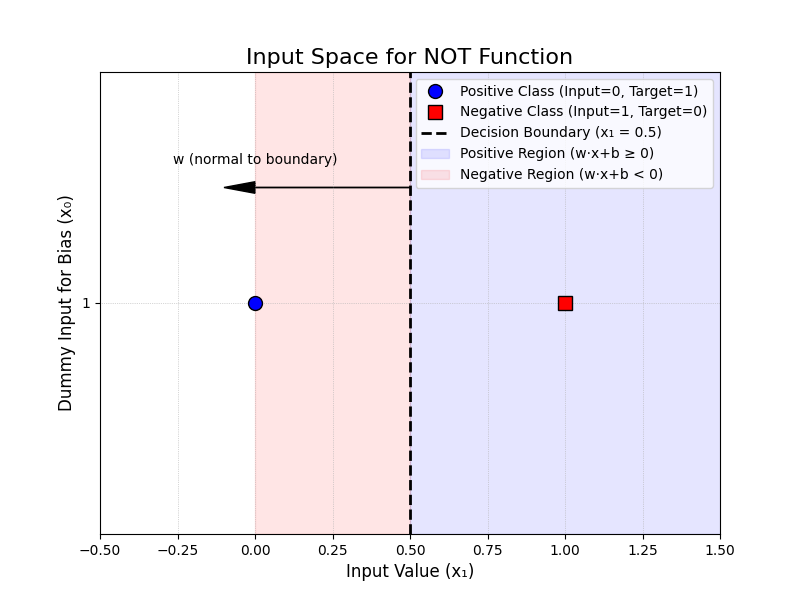
\includegraphics[width=0.6\textwidth]{not_input_space.png}
\caption{Input Space for the NOT Function.}
\end{figure}

\subsubsection{The Weight Space}
While the input space plots the data, the \textbf{Weight Space} plots the possible solutions. The axes of this space are the weights themselves. Every point in this space represents a different Perceptron model.
\begin{figure}[h!]
\centering
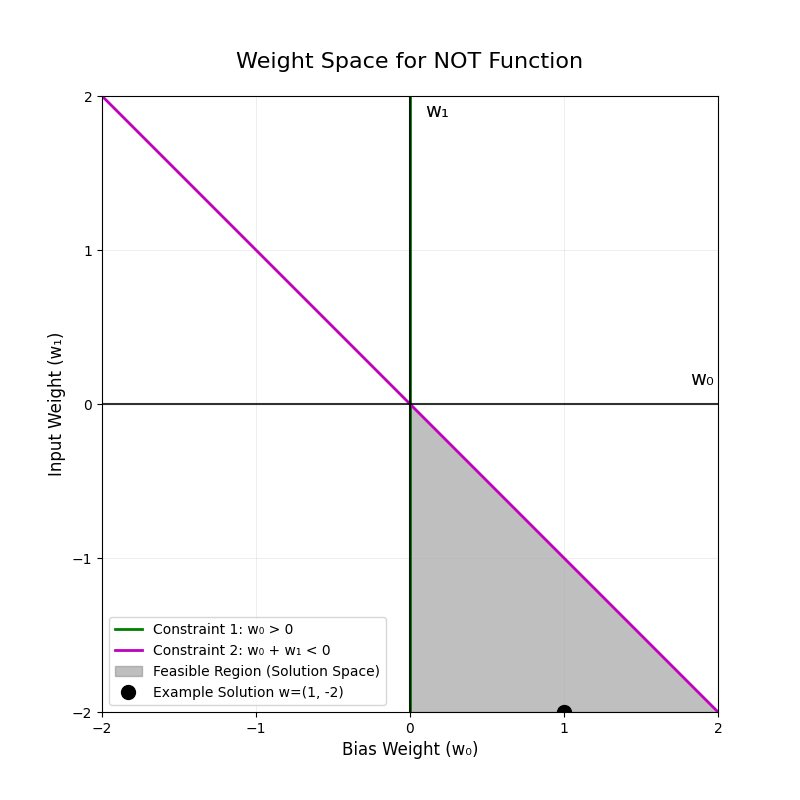
\includegraphics[width=0.6\textwidth]{not_weight_space.png}
\caption{Weight Space for the NOT Function.}
\end{figure}

\subsection{Example: The AND Function}
\subsubsection{The Input Space}
The Input Space shows our data points and the decision boundary that separates them. For the AND function, we have three "negative" points (target=0) and one "positive" point (target=1).
\begin{figure}[h!]
\centering
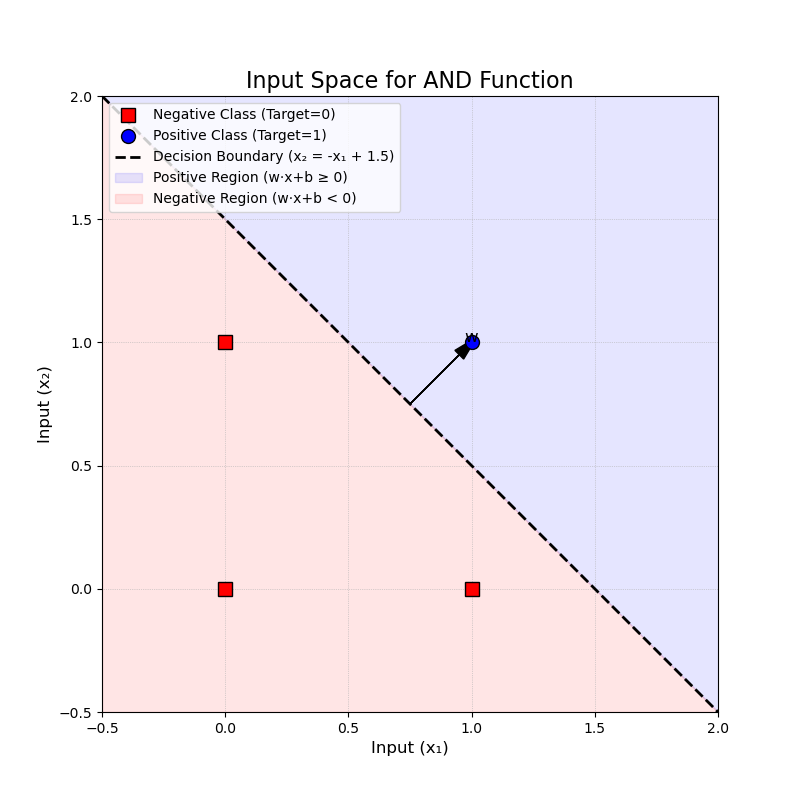
\includegraphics[width=0.6\textwidth]{and_input_space.png}
\caption{Input Space for the AND Function.}
\end{figure}

\subsubsection{The Weight Space}
The Weight Space represents the set of all possible solutions. Each of our four data points imposes a constraint on the possible values of the weights.
\begin{figure}[h!]
\centering
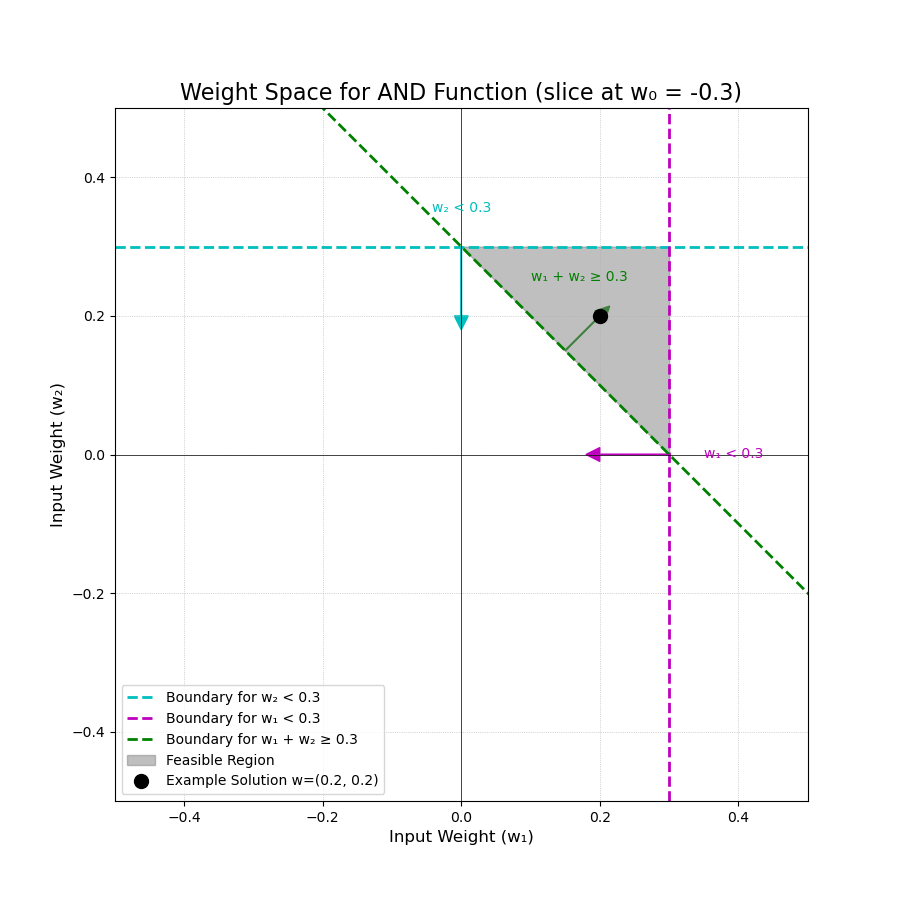
\includegraphics[width=0.6\textwidth]{and_weight_space.png}
\caption{A 2D slice of the Weight Space for the AND Function, with \(w_0 = -0.3\).}
\end{figure}

\section{Limitations of the Perceptron}
\subsection{Linear Separability Constraint}
The fundamental limitation of the perceptron is that it can only learn linearly separable functions.

\subsubsection{Definition: Linear Separability}
A dataset is \textbf{linearly separable} if there exists a hyperplane that perfectly separates the positive and negative examples:
\[\exists \mathbf{w}, b : y_i(\mathbf{w}^T \mathbf{x}_i + b) > 0 \quad \forall i\]

\subsubsection{The XOR Problem (Minsky \& Papert, 1969)}
Consider the XOR function:
\begin{center}
\begin{tabular}{|c|c|c|}
\hline
\(x_1\) & \(x_2\) & XOR \\
\hline
0 & 0 & 0 \\
0 & 1 & 1 \\
1 & 0 & 1 \\
1 & 1 & 0 \\
\hline
\end{tabular}
\end{center}

\textbf{Mathematical Proof of Non-Linear Separability}:
Assume there exists a linear classifier \(\mathbf{w}^T \mathbf{x} + b = 0\) that separates XOR data.
For the four points, we need:
\begin{align}
w_1 \cdot 0 + w_2 \cdot 0 + b &< 0 \quad \text{(point (0,0))} \\
w_1 \cdot 0 + w_2 \cdot 1 + b &> 0 \quad \text{(point (0,1))} \\
w_1 \cdot 1 + w_2 \cdot 0 + b &> 0 \quad \text{(point (1,0))} \\
w_1 \cdot 1 + w_2 \cdot 1 + b &< 0 \quad \text{(point (1,1))}
\end{align}

From equations (1) and (2): \(b < 0\) and \(w_2 + b > 0 \Rightarrow w_2 > -b > 0\)
From equations (1) and (3): \(b < 0\) and \(w_1 + b > 0 \Rightarrow w_1 > -b > 0\)
From equation (4): \(w_1 + w_2 + b < 0\)

But this contradicts \(w_1 > -b\) and \(w_2 > -b\), since:
\[w_1 + w_2 + b > -b + (-b) + b = -b > 0\]

Therefore, no linear separator exists for XOR.

\subsection{Solutions to Linear Separability Limitation}
\subsubsection{Multi-Layer Perceptrons (MLPs)}
\begin{itemize}
    \item Add hidden layers with non-linear activation functions
    \item Can approximate any continuous function (Universal Approximation Theorem)
    \item Require more sophisticated training algorithms (backpropagation)
\end{itemize}

\subsubsection{Feature Engineering}
\begin{itemize}
    \item Transform input space to make data linearly separable
    \item For XOR: Add feature \(x_3 = x_1 \oplus x_2\) (though this requires knowing the solution)
    \item Kernel methods: Implicitly map to higher-dimensional spaces
\end{itemize}

\subsubsection{Ensemble Methods}
\begin{itemize}
    \item Combine multiple linear classifiers
    \item Voting or weighted combination schemes
    \item Can learn non-linear decision boundaries
\end{itemize}

\section{Historical Impact and Legacy}
\subsection{The Perceptron Controversy}
The 1969 book "Perceptrons" by Minsky and Papert highlighted the limitations of single-layer perceptrons, leading to:
\begin{itemize}
    \item \textbf{AI Winter}: Reduced funding and interest in neural networks
    \item \textbf{Focus shift}: Emphasis moved to symbolic AI and expert systems
    \item \textbf{Delayed progress}: Multi-layer networks existed but lacked efficient training methods
\end{itemize}

\subsection{Modern Relevance}
Despite limitations, perceptrons remain important because:
\begin{itemize}
    \item \textbf{Building blocks}: Neurons in modern deep networks are perceptron variants
    \item \textbf{Theoretical foundation}: Understanding linear classifiers is crucial
    \item \textbf{Computational efficiency}: Still useful for linearly separable problems
    \item \textbf{Online learning}: Perceptron learning rule works in streaming settings
\end{itemize}

\section{Exercises} 
 
\begin{enumerate}
    \item Determine the weights of a network with 4 input and 2 output units using Perceptron learning law
\end{enumerate}
Input:
\(\begin{pmatrix} 1 & 1 & 0 & 0 \\ 1 & 0 & 0 & 1 \\ 0 & 0 & 1 & 1 \\ 0 & 1 & 1 & 0 \end{pmatrix}\)
Output:
\( \begin{pmatrix} 1& 1 & 1 & 0 & 0 \end{pmatrix} \)


\end{document}

